\documentclass{beamer}

\usepackage[british]{babel}
\usepackage{graphicx,hyperref,ru,url}
\usepackage{float}
% The title of the presentation:
%  - first a short version which is visible at the bottom of each slide;
%  - second the full title shown on the title slide;
\title[Brain Racer]{
  Brain Racer}

% Optional: a subtitle to be dispalyed on the title slide

\usepackage{subfigure}
\usepackage[export]{adjustbox}
% The author(s) of the presentation:
%  - again first a short version to be displayed at the bottom;
%  - next the full list of authors, which may include contact information;
\author[Stef, H\'ector, Thomas]{Stef Janssen\\H\'ector van den Boorn\\Thomas van Heyningen }

\begin{document}

\begin{frame}
  \titlepage
\end{frame}


% Section titles are shown in at the top of the slides with the current section 
% highlighted. Note that the number of sections determines the size of the top 
% bar, and hence the university name and logo. If you do not add any sections 
% they will not be visible.


\section{Project}
\begin{frame}
  \frametitle{Problem Description}

  Cybathlon: robust zero training classifier

  \begin{figure}
   
    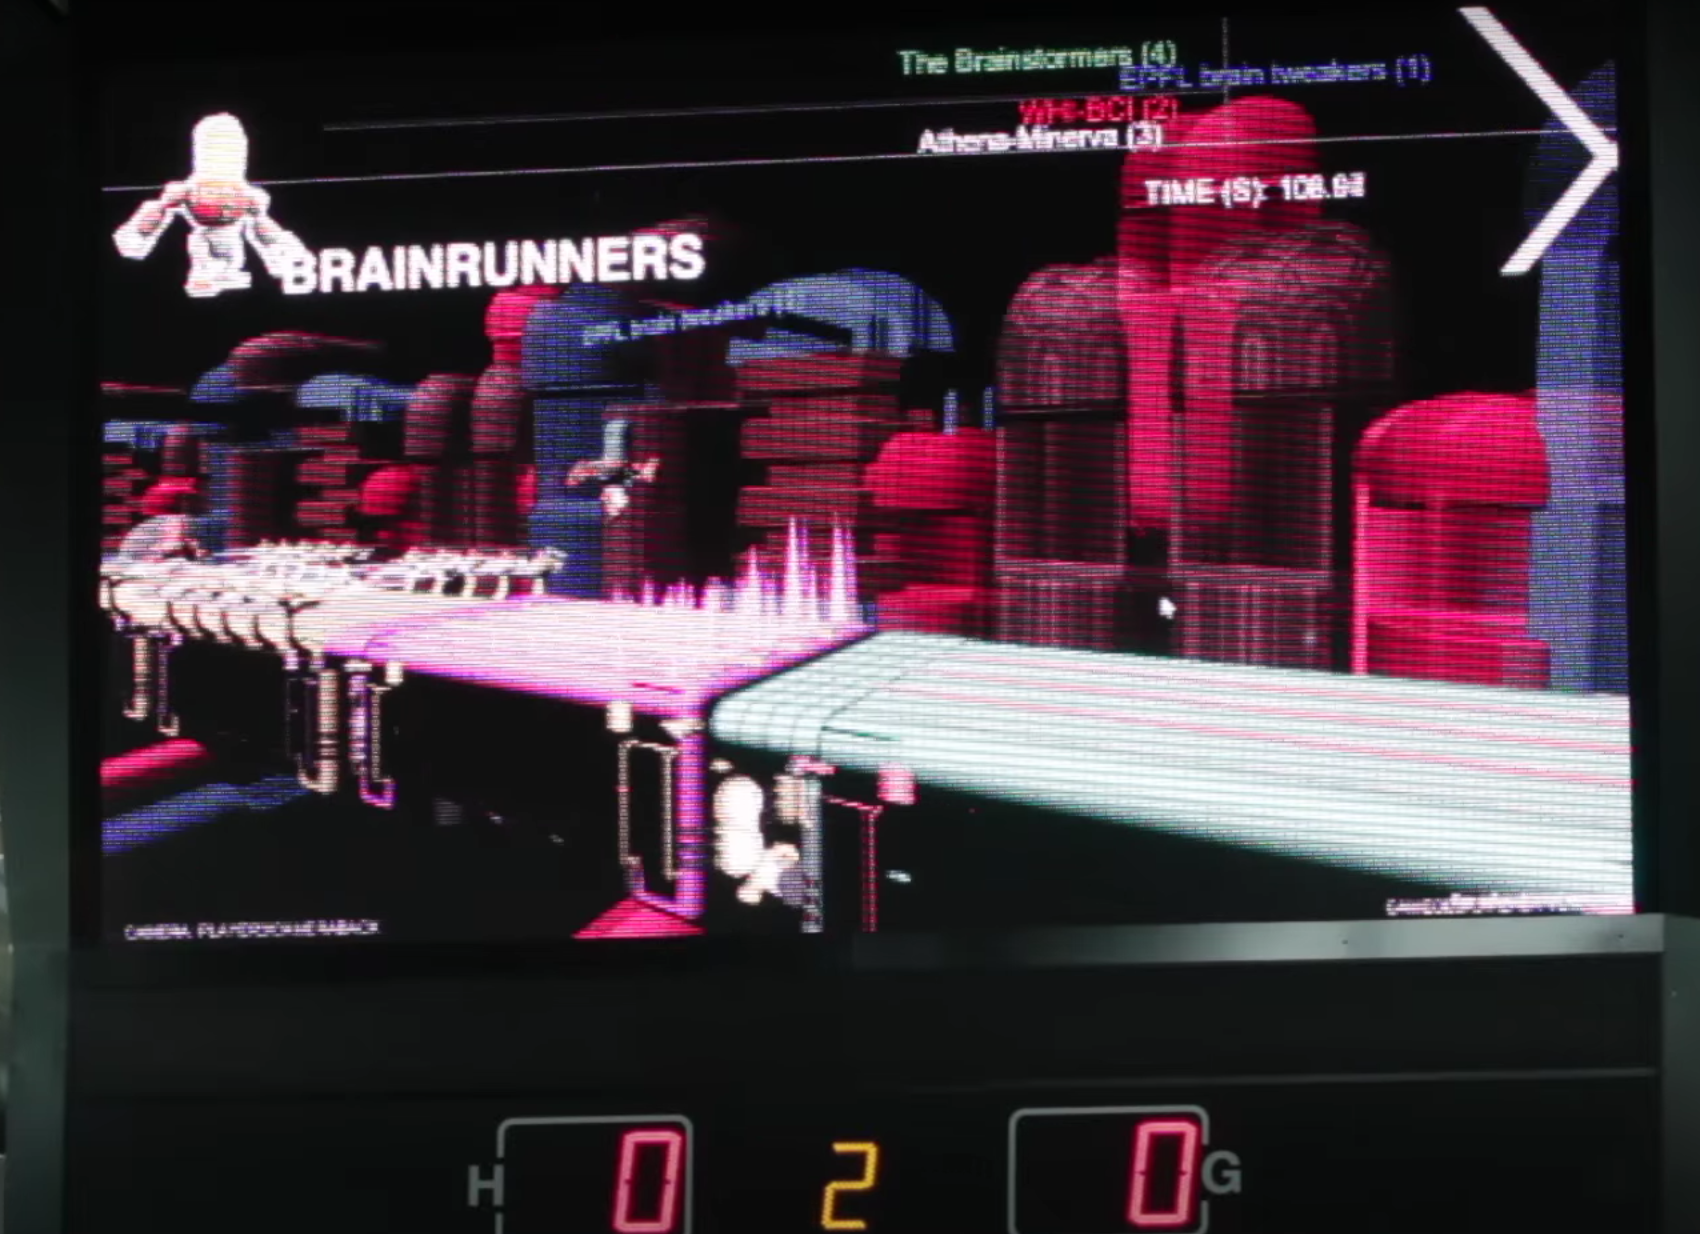
\includegraphics[width=0.5\textwidth]{cybathlon_challenge.png}
  \end{figure}
  
%Ligt toe: simpeler gemaakt naar binaire classificatie
\end{frame}

\begin{frame}
  \frametitle{Foreseen challenges}

  \begin{itemize}
    \item Covariate shift (Bickel et al., 2009)
\begin{itemize}
 \item between
 \item within
\end{itemize}
    \item EEG-performance in general (actual movement (Blokland et al., under review))
    \item Online classification
  \end{itemize}
\end{frame}

\section{Classification scheme}

\begin{frame}
  \frametitle{BCI cycle}
  \begin{figure}
    \centering
    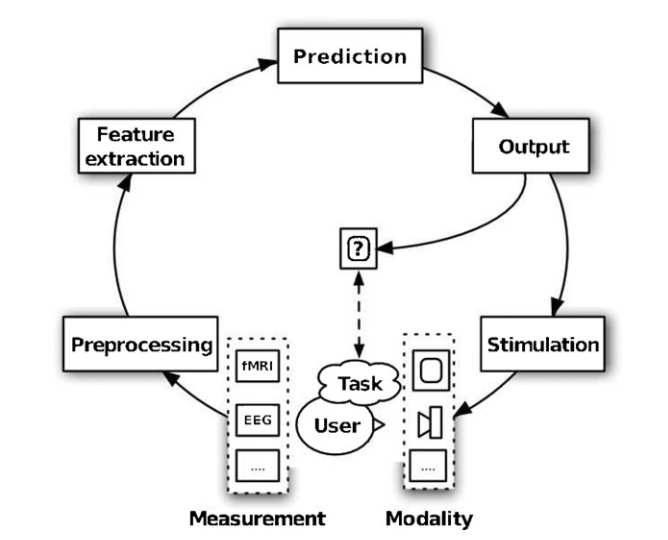
\includegraphics[width=0.7\textwidth]{bci_cycle.png}
  \end{figure}
 
\end{frame}

\begin{frame}
  \frametitle{Preprocessing + Feature Extraction}

  \begin{columns}

  \begin{column}{0.5\textwidth}
      \begin{itemize}
    \item Preprocessing 
	\begin{itemize}
		\item Channel selection
		\item Spatial filter
		\item Detrending
		\item Windowing
	\end{itemize}
	 
    \item Feature Extraction
	\begin{itemize}
		\item Welch's method
		\item $\mu$ and $\beta$ frequencies
	\end{itemize}
  \end{itemize}

  \end{column}
 
  \begin{column}{0.5\textwidth}
     \begin{figure}
  \centering
     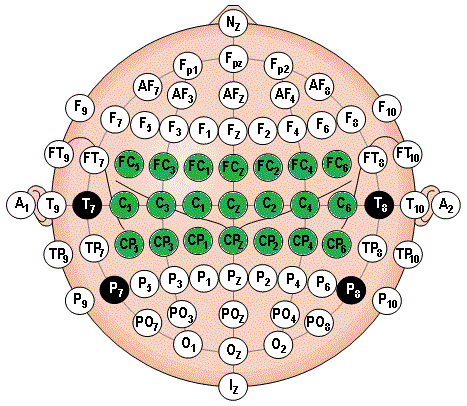
\includegraphics[width=0.8\textwidth]{cap.png}
 \end{figure}
  \end{column}
\end{columns}

\end{frame}

\begin{frame}
  \frametitle{Classification Pipeline}
  
  \begin{itemize}
    \item KMeans
    \item Multivariate Gaussian EM
    \item PCA
    \item Logistic Regression
  \end{itemize}
  Performance?
\end{frame}

\begin{frame}
  \frametitle{Classification Pipeline}
    \begin{columns}

  \begin{column}{0.5\textwidth}
\begin{itemize}
    \item KMeans     
    \item Multivariate Gaussian EM
    \item PCA
    \item Logistic Regression
  \end{itemize}

  \end{column}
 
  \begin{column}{0.5\textwidth}
  \begin{figure}
    
\includegraphics[width=0.8\textwidth, right]{chucktesta.jpeg}
  \end{figure}
  \end{column}
\end{columns}
 \vfill
    Classification at chance level $\rightarrow$ plan B: ERSP classifier with adaptive LR.

\end{frame}
\section{Experiment setup}
\begin{frame}
  \frametitle{Stimulation}

  \begin{figure}
    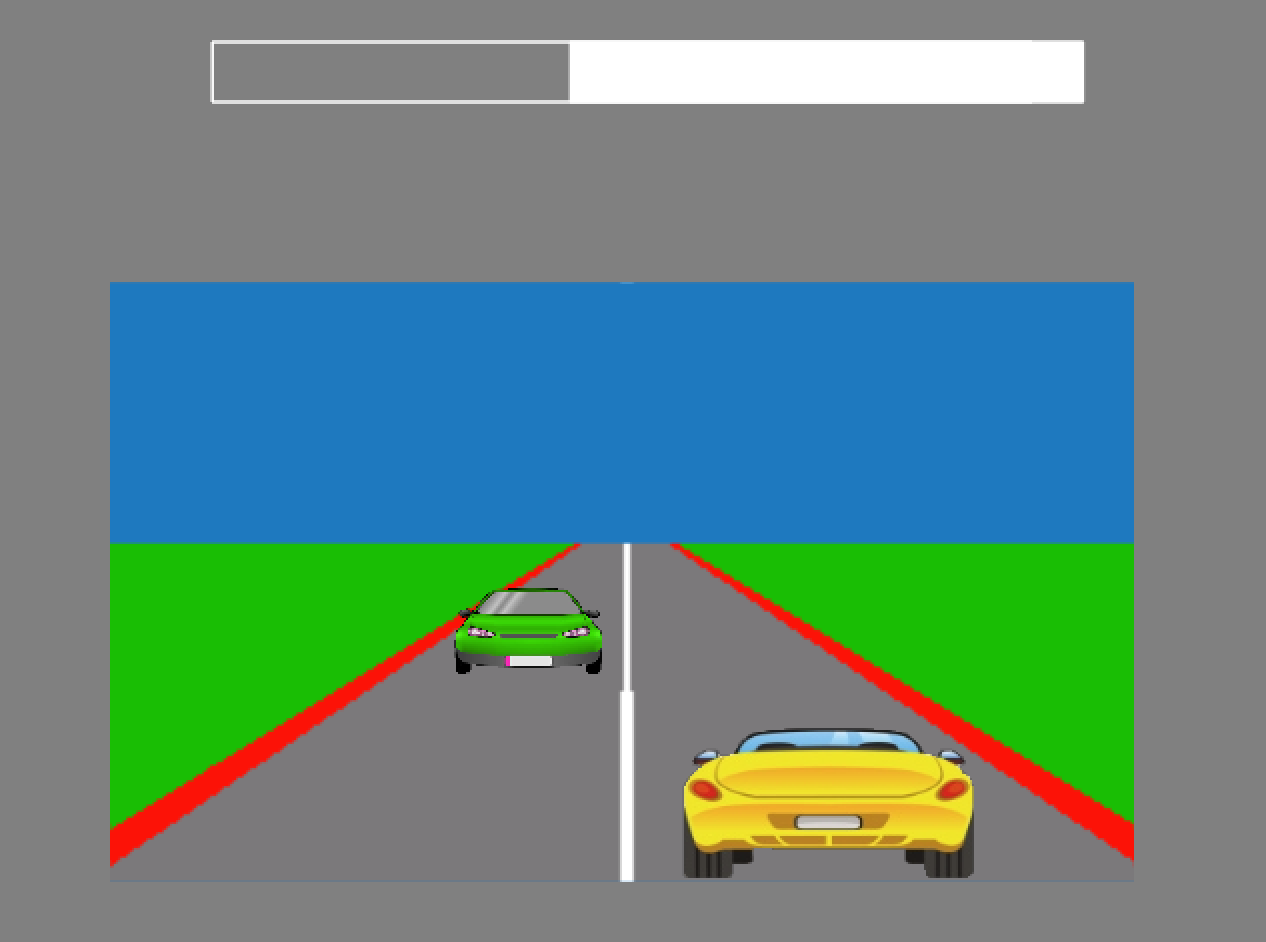
\includegraphics[width=0.7\textwidth]{brain_racer.png}
  \end{figure}

\end{frame}



\begin{frame}
  \frametitle{Pipeline}

  \begin{figure}
    \centering
    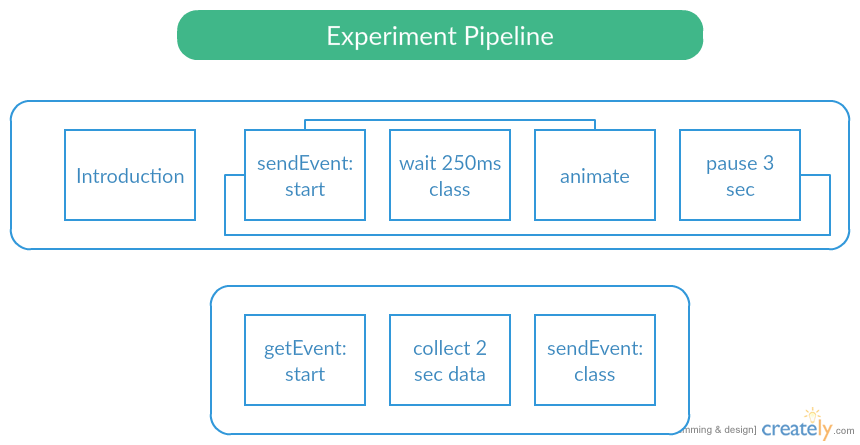
\includegraphics[width=0.9\textwidth]{brain_racer_pipeline.png}
  \end{figure}
\end{frame}

\section{Results}

\begin{frame}
  \frametitle{Class distinctiveness}

 \begin{figure}
  \centering
     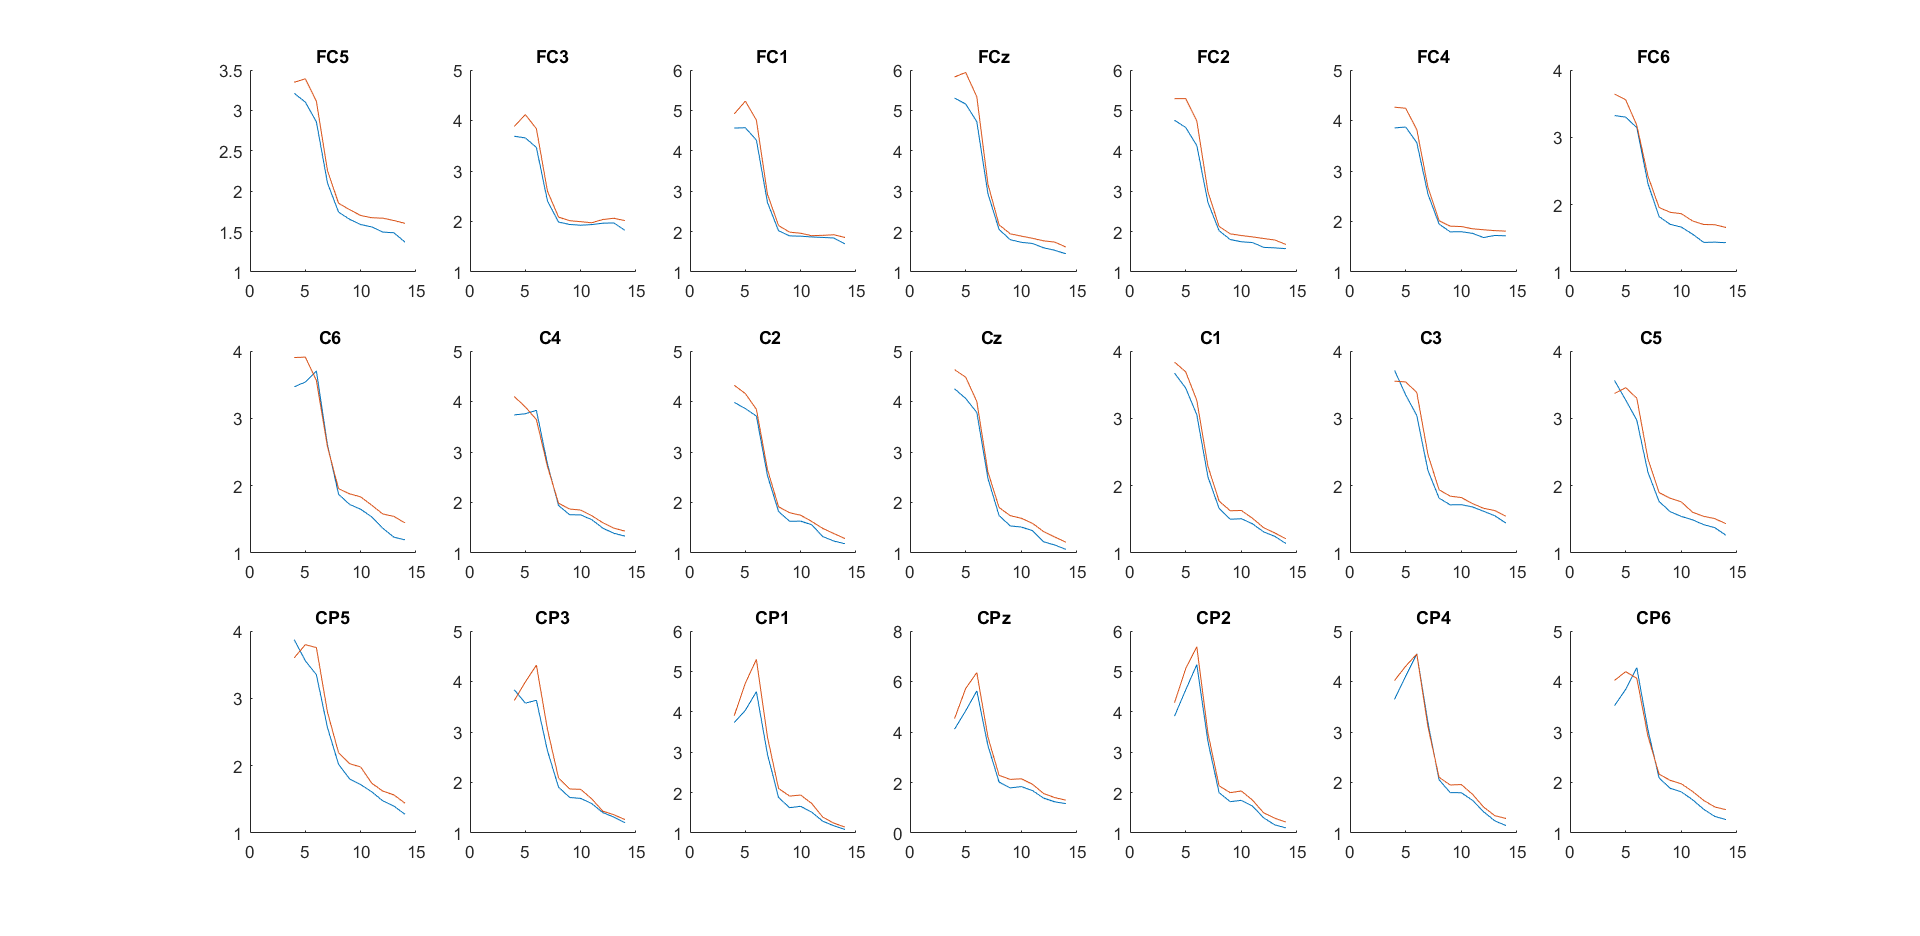
\includegraphics[width=1.0\textwidth]{distinction.png}
 \end{figure}

\end{frame}

\begin{frame}

\frametitle{2 ways of validating}
 \begin{itemize}
   \item Between: Trained on 2 $\rightarrow$ tested on 1
   \item Within: Cross validated on each subject
 \end{itemize}

\end{frame}

\begin{frame}
  \frametitle{Results}

 \begin{figure}
  \centering
     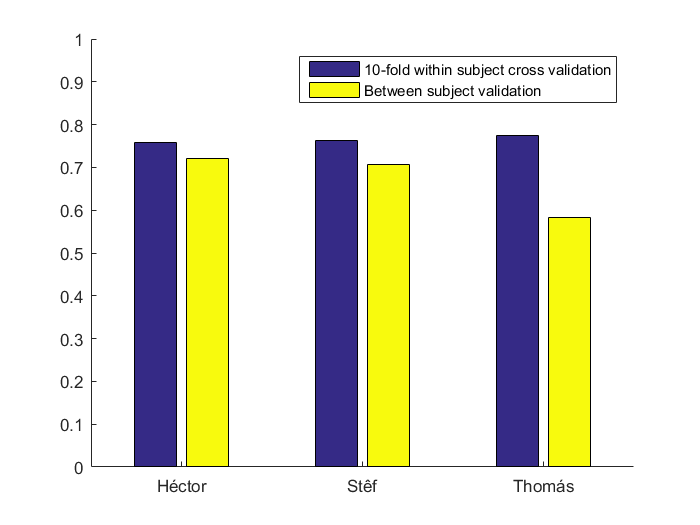
\includegraphics[width=0.7\textwidth]{bars.png}
 \end{figure}

\end{frame}

\section{Discussion}
\begin{frame}

\frametitle{Take Home Message}
  \begin{itemize}
   \item Adaptive approach produced slightly better results
   \item More subjects and sessions needed to build prior
  \end{itemize}
\end{frame}

\end{document}
